\chapter{Implementación}
{\color{blue}



La implementación de la aplicación se realiza con \textbf{Kaa IoT} tal y como se analizo anteriormente \ref{eleccion-framework}. Para empezar a usar el framework, hay que registrarse en sistema. Una vez registrados tendremos acceso a nuestro \textit{dashboard} \footnote{Hace referencia al cuadro de mandos al que tenemos acceso para interactuar con nuestro dispositivo y todas las posibles configuraciones}. En este capítulo se trata de mostrar una guía con la que se consiga conectar un dispositivo, recoger y enviar datos desde/hacia el dispositivo y mostrar las opciones que nos ofrece Kaa IoT como framework IoT. Para empezar, vamos a conectar nuestro primer dispositivo.

\begin{figure}[hb!]
    \centering
    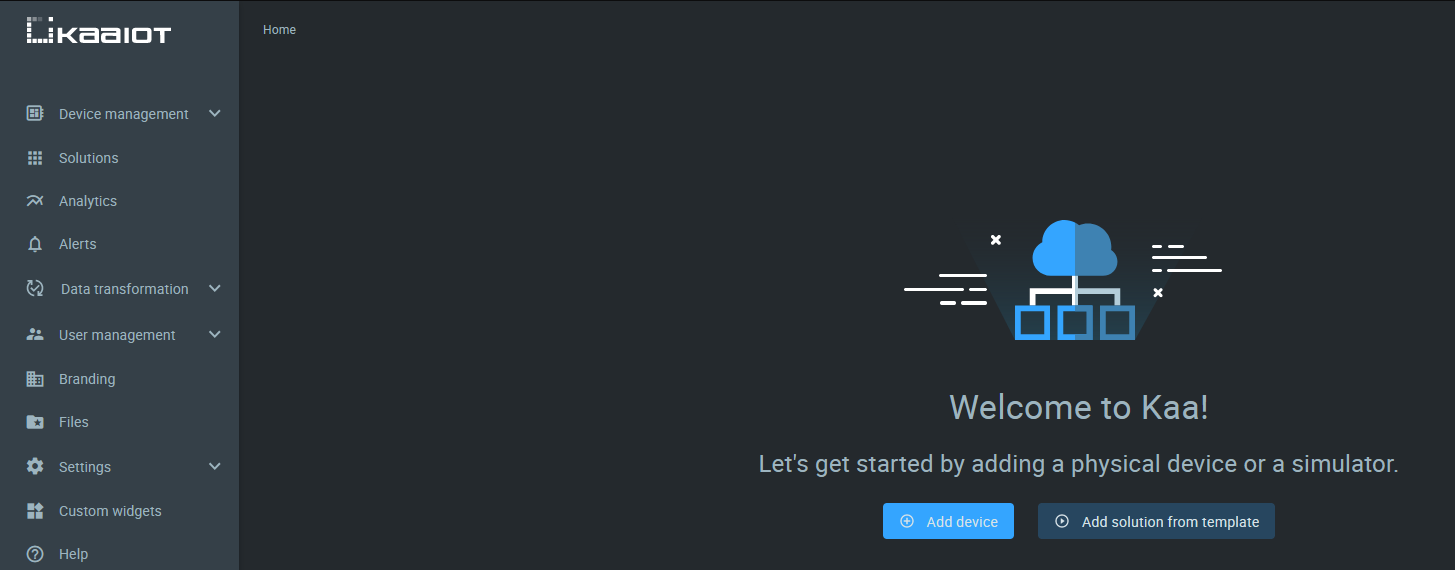
\includegraphics[width=\linewidth]{imagenes/dashboard.png}
    \caption{Dashboard Kaa IoT.}
    \label{fig:figure5}
\end{figure}


\section{Conectar dispositivo}

En este apartado se trata de explicar el proceso de conexión de un dispositivo con nuestra aplicación, desde crear un endpoint hasta ver la información del dispositivo en nuestra interfaz de usuario. Esto engloba varios términos y conceptos que se van a definir a continuación.

\subsection{Términos y conceptos}

\subsubsection{Endpoints}

Los endpoints representan ``el elemento de las cosas`` del IoT. Un endpoint es cualquier dispositivo terminal que se quiera gestionar, en nuestro caso desde Kaa IoT. Un endpoint puede ser un dispositivo físico o una emulación de software del mismo. Todos los datos que llegan a la aplicación están asociados a endpoints. \cite{kaaiotConcepts}

Para ser precisos, un endpoint puede ser una unidad menor que un dispositivo, lo que significa que un dispositivo físico puede incluir múltiples endpoints. Por ejemplo, quieres gestionar un termostato, para que el aire acondicionado se encienda y apague automáticamente a cierta temperatura.

Se puede gestionar el termostato de una de las siguientes maneras:

\begin{itemize}
    \item Toda la unidad del termostato actúa como un endpoint único que intercambia datos con el servidor.
    \item Los componentes del termostato, como los sensores de temperatura y humedad, interruptor de encendido/apagado, actúan como endpoints individuales.
\end{itemize}

\subsubsection{ID de Endpoint}

El ID de endpoints se utiliza para identificar de forma única un endpoint dentro de una instancia. Un ID de endpoints suele ser un UUID generado automáticamente por el framework en el momento de crear un nuevo endpoint. No obstante, también se permiten los ID de endpoints definidos por el usuario. El ID de los endpoints no puede modificarse una vez creado.

Todos los datos de los endpoints, como los atributos de los metadatos, los puntos de datos de series temporales recopilados, los comandos, etc., están asociados a un ID de endpoint específico. Siempre que recupere o gestione datos relacionados con endpoints en Kaa, principalmente a través de la API REST, se verá los ID de endpoints.

}